\clearpage
\section{雾中的点光源}
Sponza 的三盏点光源悬在走廊上方。左图里，读者主要从柱面和挂毯的亮度判断灯在何处。右图里，连灯前面的空气也亮了起来。两个画面用同一组灯和相机。打开 Vulkan 编辑器，在「实时效果」里勾选「体积雾」，就可以在组合光照 Lit 里看见这个变化。

\begin{center}
\begin{minipage}{.485\linewidth}\centering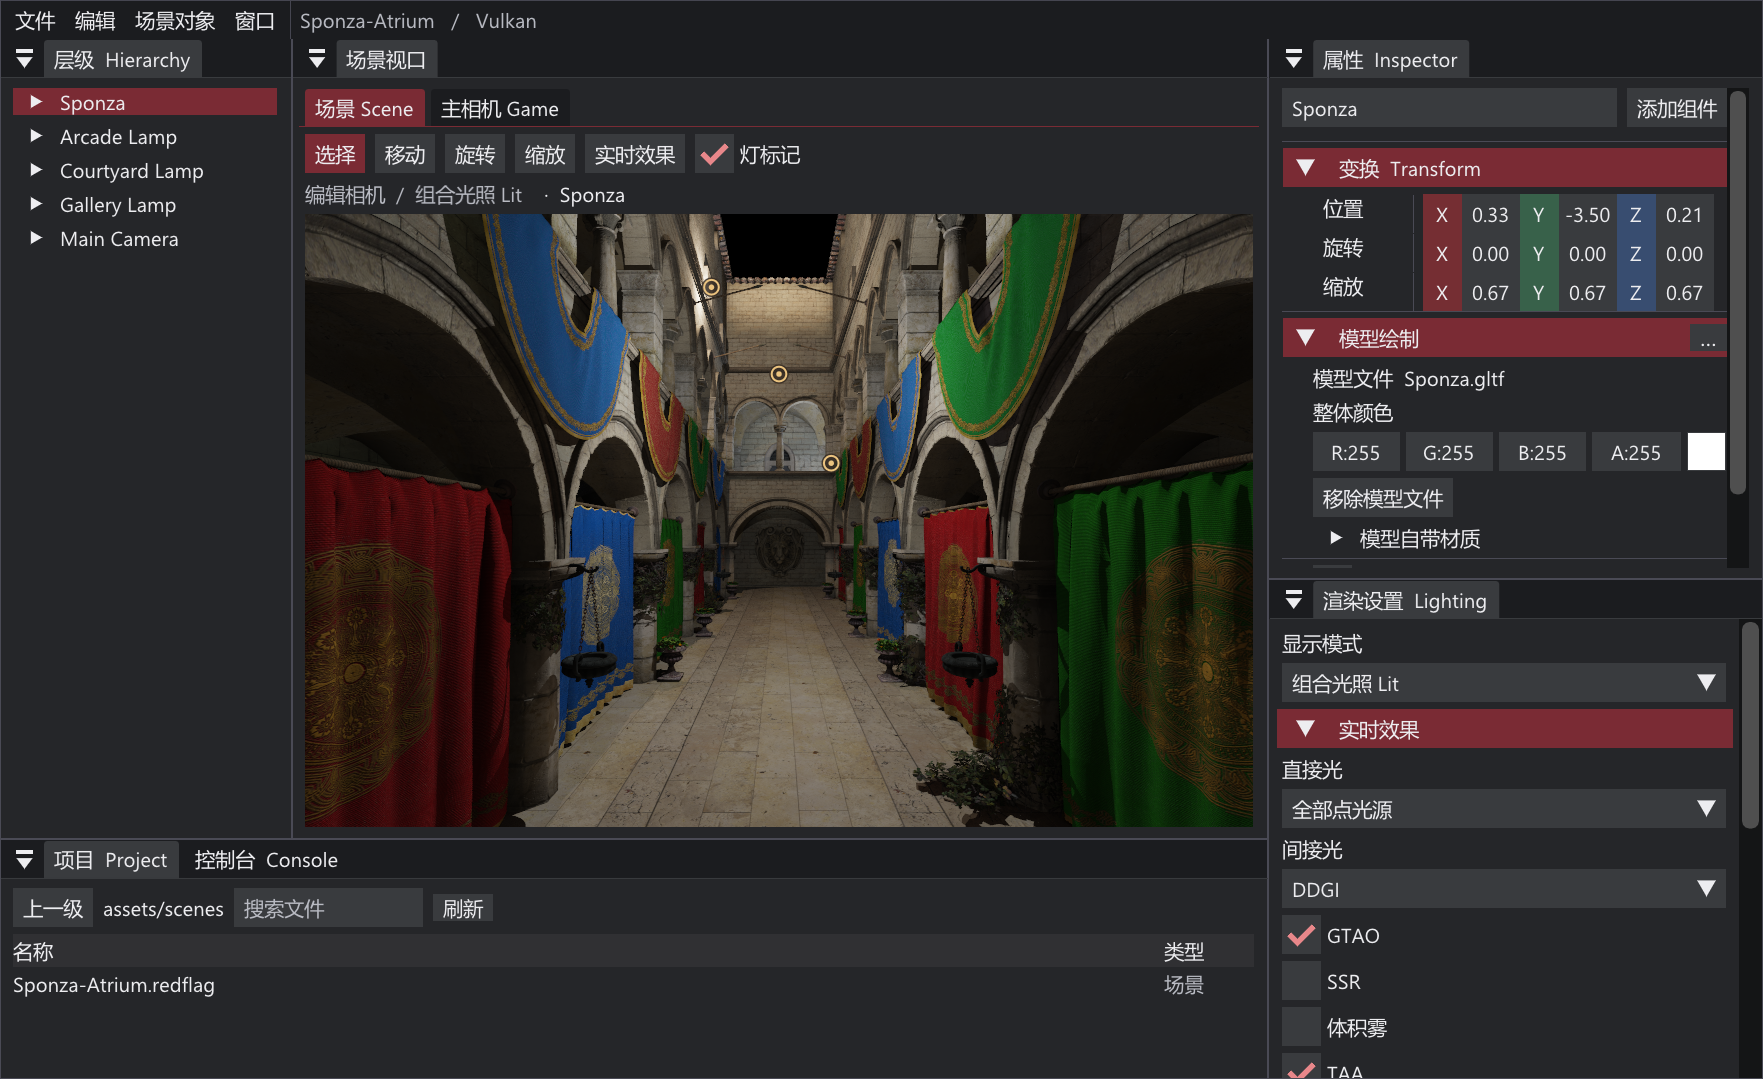
\includegraphics[width=\linewidth,trim=305bp 252bp 510bp 214bp,clip]{../../../output/profiling/fog/sponza-clear.png}\\{\small 体积雾关闭}\end{minipage}\hfill
\begin{minipage}{.485\linewidth}\centering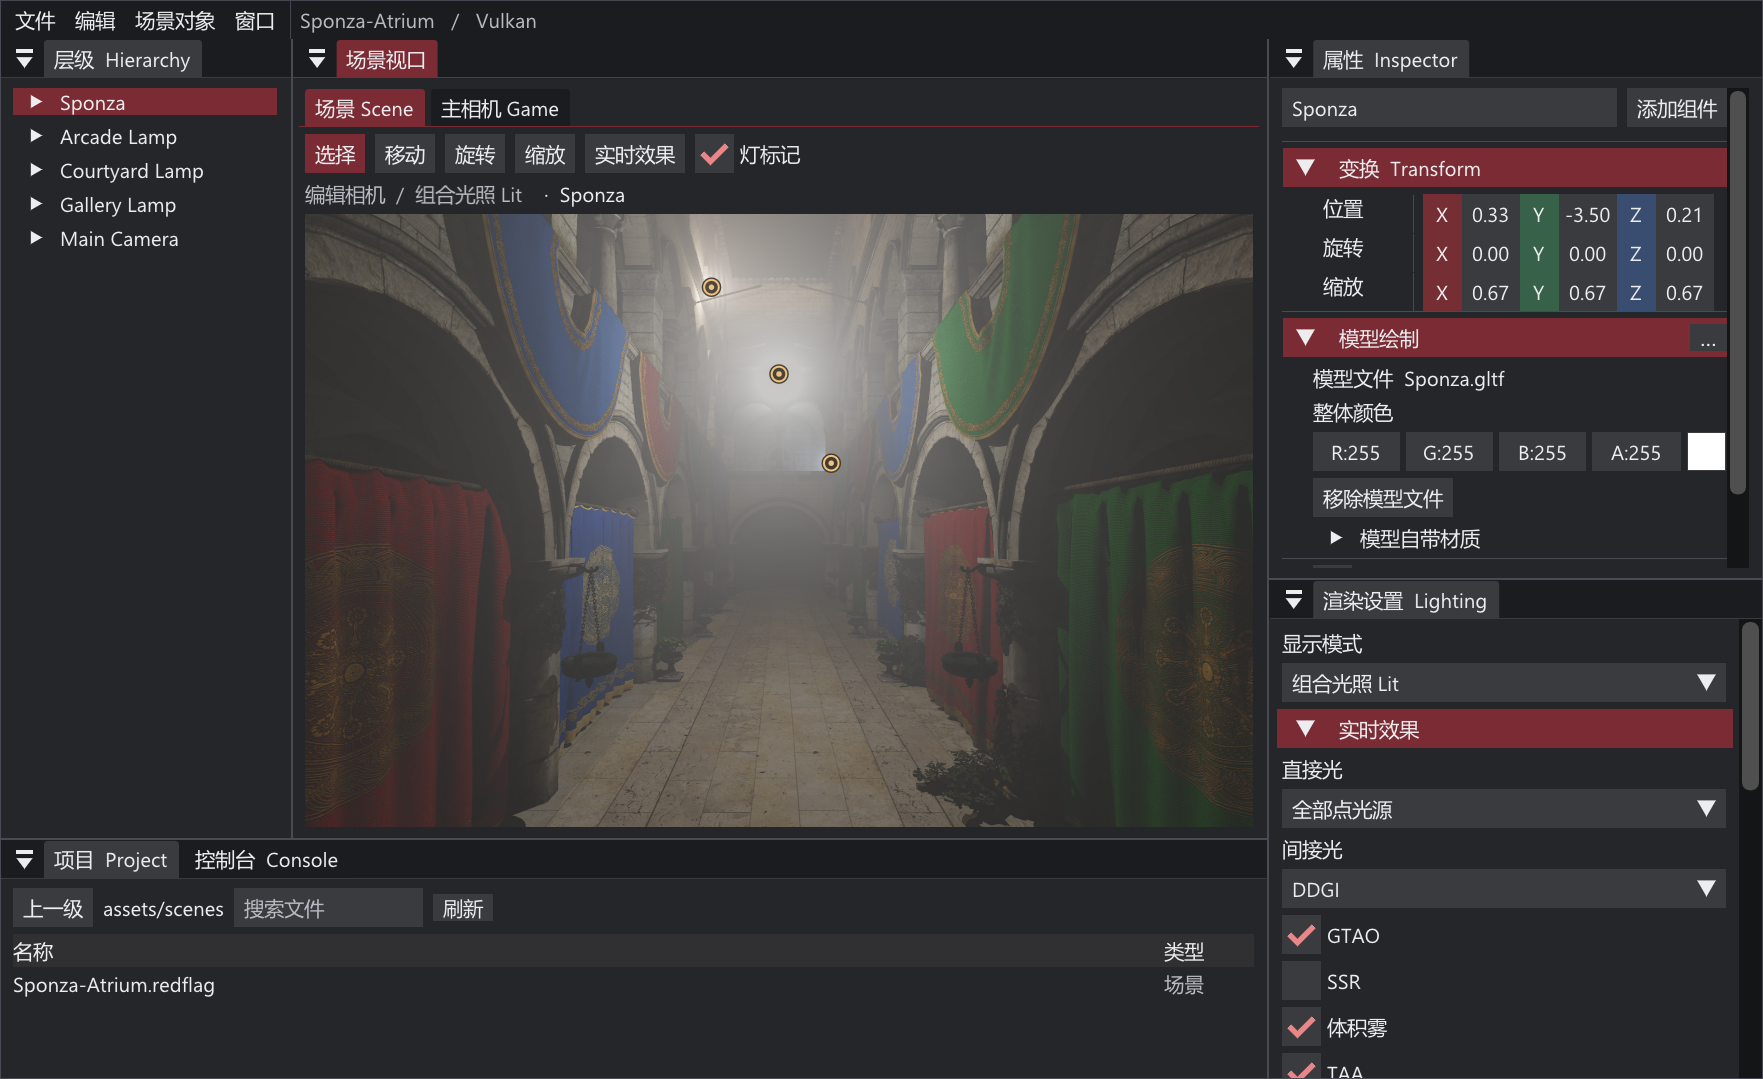
\includegraphics[width=\linewidth,trim=305bp 252bp 510bp 214bp,clip]{../../../output/profiling/fog/sponza-fog.png}\\{\small 体积雾开启}\end{minipage}
\end{center}
{\small\color{quiet}Redflag 正式 Vulkan 编辑器，$948\times613$。雾密度 0.10，散射比例 0.92，散射方向 0.35，最远距离 24，16 步。}

先看远端的拱门。表面反射的光要穿过空气才到达镜头。假设穿过一个世界单位后还剩原来的 90.5\%，穿过两段就剩 $0.905^2$。把雾密度记作 $\sigma_t$，距离记作 $d$，穿过整段后能保留的比例为 $T(d)=\exp(-\sigma_t d)$。取右图的 $\sigma_t=0.10$，一段长 10 的路只剩 $e^{-1}\approx0.368$。面板中的「雾密度」使用每世界单位的消光系数，场景若按米建模，单位就是每米。

再看灯附近的白雾。有些光离开点光源，还没碰到地面便被雾滴散射，其中一部分转向镜头。程序沿一个像素的视线取样。若采样点与灯之间隔着墙，该灯就照不到这里。穿过窗洞的光只照亮那些能看见灯的采样点，于是雾里出现一束带轮廓的光。

\begin{center}
\begin{tikzpicture}[font=\small,>=stealth]
\draw[fill=shade,draw=quiet!40,rounded corners] (0,0) rectangle (13.4,2.55);
\node at (1.0,.44){镜头};\node at (11.9,.44){可见表面};
\draw[->,very thick,wine] (1,.85)--(11.8,.85);
\foreach \x in {2.4,4.4,6.4,8.4,10.4}{\fill[wine] (\x,.85) circle (2.4pt);}
\node at (5.5,2.18){点光源};\draw[->,quiet] (5.5,1.97)--(4.45,.94);
\draw[dashed,quiet] (5.8,1.98)--(8.35,.9);
\draw[line width=2pt] (7.2,1.05)--(7.2,1.8);
\node[fill=shade,inner sep=1pt] at (9.25,1.86){墙挡住了右侧的光};
\end{tikzpicture}
\end{center}
{\small\color{quiet}本册绘制。红点是每一小段的中点。视线在最近的表面结束，穿墙之后的雾不会叠在墙前。}

\clearpage
\subsection*{沿视线积累光照}
把长度 $d$ 切成 $N$ 段，每段长 $h=d/N$。设 $a$ 为单次散射比例，$L_s$ 为中点处从各盏灯到达、并按散射方向加权后的入射亮度。单段中，直线传过的比例是 $t=e^{-\sigma_t h}$，离开原来方向的比例就是 $1-t$。把入射亮度近似看成这一小段内恒定，散射到镜头方向的增量是 $a(1-t)L_s$。它还要穿过镜头与该段之间的雾。第 $j$ 段从零计数，最后的像素为
\[
 L_{\rm pixel}=t^N L_{\rm surface}
   +\sum_{j=0}^{N-1}t^j\, a(1-t)\,L_{s,j}.
\]
\noindent{\small\color{quiet}按 GLSL 整理的伪代码\quad\href{run:../../Redflag/src/Redflag/Renderer/GI/Shaders/Fog.comp}{\texttt{Fog.comp}}}\par\nopagebreak
\begin{lstlisting}[escapeinside={(*@}{@*)}]
T = 1; scattered = 0
for each segment from the camera:
    point = midpoint(segment)
    incident = sum_visible_point_lights(point, viewRay)
    (*@{\footnotesize\color{quiet}这一段散向镜头的光，还要穿过前面各段雾。}@*)
    scattered += T * albedo * (1 - stepT) * incident
    T *= stepT
output = scattered + T * surfaceColor
\end{lstlisting}

例如一层雾让 80\% 的表面光穿过，散射比例为 0.75。设这层雾从可见灯光得到的方向加权亮度为 2，朝镜头散射的增量就是 $0.75\times0.2\times2=0.3$。若它的前面还有一层同样的雾，到达镜头的这份增量会降到 $0.8\times0.3=0.24$。程序中的 \texttt{T} 便是沿途这些比例的乘积。

\pair{profiling/fog/open.png}{点光源穿过方孔}{profiling/fog/closed.png}{同一盏灯，方孔封住}
{\small\color{quiet}同一个 Vulkan 离屏场景，$384\times216$，32 步。右半部中央的取样位置在左上角起算的 $(288,108)$；封住小孔后，这里的线性红色分量从 0.02275 降为 0。}

\clearpage
\subsection*{编辑器中的取值与检查}
雾较稀时，可以先把「雾密度」设为 0.03，把「散射方向」设为 0，这样从各个方向观察同一团雾都使用相同的散射权重。想让逆光更明显，可逐步调高散射方向。它控制 Henyey--Greenstein 相函数中的 $g$，也就是入射方向与散射后方向之间的平均余弦。正值偏向继续向前传播的光，负值偏向散回光源一侧。着色器使用
\[
p_g(c)=\frac{1-g^2}{4\pi(1+g^2-2gc)^{3/2}},
\qquad c=\hat{\boldsymbol l}\cdot\hat{\boldsymbol v}.
\]
单位向量 $\hat{\boldsymbol l}$ 从采样点指向灯，$\hat{\boldsymbol v}$ 从镜头指向采样点。它们都和光实际旅行的方向相反，一起取反不改变点积。灯到采样点这段还要乘 $e^{-\sigma_t r}$ 和距离平方的倒数，$r$ 是到灯的距离。每盏灯沿用点光源属性中的半径，雾与表面在同一半径外都收不到这盏灯的光。实现将平方距离的最小值取为 $0.04$，相当于在距点光源 0.2 个单位以内限制亮度，避免单个采样点恰落在灯心时失控。

\begin{fields}
\texttt{FogSettings} & 保存密度、散射比例、散射方向、最远距离和步数。体积雾默认关闭，打开后这些值跟随场景的 \texttt{.render.yaml} 保存。\\
\texttt{RenderFog} & 接收线性场景颜色。每个像素用 \texttt{GISurface} 找到最近表面；背景沿视线算到最远距离或相机远平面。\\
\texttt{Fog.comp} & 中点到每盏点光源的遮挡使用场景三角形的层次包围盒。结果先交给 TAA，再由显示着色器调亮度。\\
\end{fields}

图中方孔测试用了恒定密度的雾。关灯、将表面输入设为白色后，画面应只剩透过来的白光。测试按各像素自己到表面的距离计算理论值，82,944 个像素中最大的绝对误差为 $3.13\times10^{-7}$。打开灯再封住方孔，照不到的区域应重新变暗。另将半径从无限缩为一个单位。镜头中央的视线距离灯约三单位，红通道从 0.299884 降到 0.244632，与关灯时相等。

缩短「雾的最远距离」会截去远处的雾。增大步数会减轻窄光束上的条带，也会增加遮挡查询。在方孔小场景中，32 步的单次计算在 RenderDoc 回放中用时约 0.41 毫秒；完整 Sponza 有更多三角形和点光源，要另行测量。这一版采用均匀介质的单次散射，表面照明仍来自已有的 Lit 计算。较浓的雾里，散射多次才到达眼睛的光还没有计入。

{\small\color{quiet}\href{https://pbr-book.org/4ed/Volume_Scattering/Transmittance}{PBRT 第四版，§11.2 Transmittance}；
\href{https://pbr-book.org/4ed/Volume_Scattering/Phase_Functions}{§11.3 Phase Functions}；
\href{https://github.com/mmp/pbrt-v4}{PBRT v4 作者源码}；
\href{https://www.realtimerendering.com/advances/s2015/index.html}{S. Hillaire，SIGGRAPH 2015 课程，Physically-based and Unified Volumetric Rendering in Frostbite}。Frostbite 课程采用分块的体积网格，本项目沿各像素的视线积分。测试入口为 \texttt{tests/run\_fog\_tests.cmd}。}
